\documentclass{article}

% packages
\usepackage[a4paper, margin=1.8cm]{geometry}
\usepackage{multicol}
\usepackage[utf8]{inputenc}
\usepackage[english]{babel}
\usepackage{minted}
\usepackage{tikz}
\usepackage{pgfplots}
\usepackage{parskip}
\usepackage{amsmath}
\usepackage{xcolor}
\usepackage[margin=2cm]{caption}
\usepackage{graphics}

\pgfplotsset{compat=1.16}

\newlength\figurewidth
\newlength\figureheight
\setlength\figurewidth{0.3\textwidth}
\setlength\figureheight{0.3\textwidth}

\begin{document}

    \begin{titlepage}
        \begin{center}
            \vspace*{2cm}
            
            {\huge \textbf{xCore-200 Cellular Automaton Farm}}
            
            \vspace{0.5cm}
            
            {\Large COMS20001 Concurrent Computing CW1}
            
            \vspace{0.5cm}
            
            {\large Team 6}
            
            \vspace{1cm}
            
            \hspace*{1cm} {\Large \textbf{Ruairi Fox}} \hfill {\Large \textbf{Liam Dalgarno}} \hspace*{1cm} \\~\\[-0.5em]
            \hspace*{1cm} MEng. Computer Science \hfill MEng. Computer Science  \hspace*{1cm} \\~\\[-1em]
            \hspace*{1cm} rf17160@bristol.ac.uk  \hfill ld17285@bristol.ac.uk  \hspace*{1cm} 
            
            \vspace{1cm}
            
            {\large \today}
        \end{center}
    \end{titlepage}

    \section{Functionality and Design}
    1 Page Max: Outline what functionality you have implemented, which problems you have solved with your implementation and how your program is designed to solve the problems efficiently and effectively
    \pagebreak

    \section{Tests and Experiments}
    (2 pages max): Show the result of the given 16x16 image after 2 rounds. Describe briefly the other experiments you carried out, provide a selection of appropriate results and output images. This must be done for at least the example images provided and for at least one example image of your own choosing (showcasing the merit of your system). List the important factors responsible for virtues and limitations of your system.
    
    \subsection{Bit Packing}

    We pack 32 cells into a single \verb|uint32| as soon as the data is read by \verb|data_in|, which reduces the memory footprint and channel congestion. The memory footprint is reduced by a factor of 8 since each cell is represented using a single bit over a \verb|uchar| which allows us to fit larger boards into memory. Channel congestion however, is reduced by a factor of 32. Beforehand, the cells were sent one at a time, but with bit packing we can send 32 cells in one message. This reduces waiting times for channel communication, and therefore increases processing speed. However, our evolution algorithm relies on both the cells being full packets and extensive bit shifting. As a result, our system does not work with images where the width is not divisible by 32.
    
    \begin{figure}[h]
        \hspace{-0.9cm}
\begin{minipage}{0.45\textwidth}
    \begin{minted}[fontsize=\footnotesize]{C}
        uint32_t pack(uchar bits[32]) {
            uint32_t packed = 0;
            for (uchar i = 0; i < 32; i++) {
                packed |= (uint32_t) (bits[i] >> 7) << (31 - i);
            }
            return packed;
        }
    \end{minted}
\end{minipage}
\hspace{0.4cm}
\begin{minipage}{0.45\textwidth}
    \begin{minted}[fontsize=\footnotesize]{C}
        void unpack(uchar result[32], uint32_t packed) {
            for (uchar i = 0; i < 32; i++) {
                result[i] = ((packed >> (31 - i)) & 0x1) * 255;
                }
            }
        }
    \end{minted}
\end{minipage}
        \caption{Bit packing code}
        \label{fig:bitpack}
    \end{figure}

    \subsection{Evolution}

    To further save on memory, our workers evolve the board `in place', i.e. there is only one copy of the board which stores both the state of the current generation and the next. This is achieved by exploiting the fact that once a row is processed, the row above is redundant, and as such we can overwrite it with the new processed row. A downside of this approach is that the next generation is shifted upwards by one row. Therefore, its necessary to shift every row back down to keep the board structure the same and make room for the overlapping rows.

    \begin{figure}[h]
        \begin{center}
            \begin{alignat*}{3}
    &\big[0101\dots1110\big]         &{}                                                                                     &\big[\textcolor{green!60!black}{0100\dots0010}\big] \\
    &\big[\textcolor{cyan!75!black}{0111\dots0110}\big] \mapsto &\big[\textcolor{green!60!black}{0100\dots0010}\big] \mapsto &\big[\textcolor{cyan!75!black}{0111\dots0110}\big] \\
    &\big[1100\dots1000\big]         &{}                                                                                     &\big[1100\dots1000\big] 
\end{alignat*}
            \caption{Processing the current row and placing it in the row above. Green: next generation row; Blue: current generation row.}
            \label{fig:rows}
        \end{center}
    \end{figure}

    \subsection{Architecture}

    Our \verb|distributor| does not store the state of the board, but passes on the work from the \verb|data_in| to the correct worker; it is then up to the workers to send their overlapping rows to each other. Without this approach, the distributor would end up storing the `initial state' of the board, which, for a \verb|1024x1024| image, would result in $1024 \cdot 32 \cdot 4 = 131072$KB of wasted memory. In fact, between generations, the workers only send their overlapping rows to each other unless it is time to export the board. This, paired with the `empty' \verb|distributor|, avoids the \verb|distributor| becoming a bottleneck for evolution since the workers can communicate in parallel. The workers are also split evenly across the tiles to minimise hard channel usage, with the first $\frac{n}{2}$ being on tile 0 and the remaining on tile 1.

    \begin{figure}[h]
        \begin{center}
            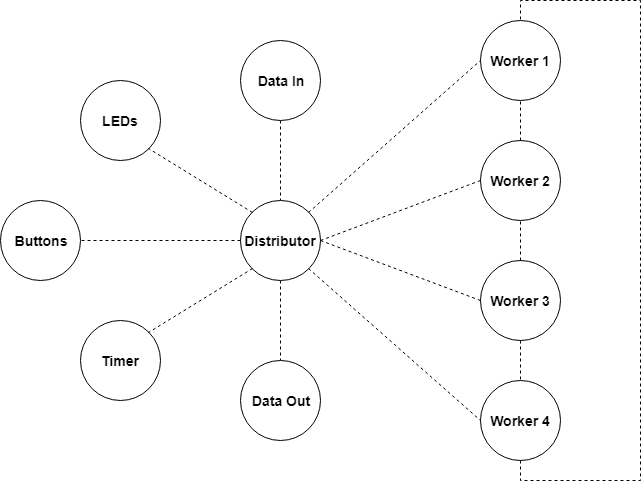
\includegraphics[width=0.6\textwidth]{architecture.png}
            \caption{High-level channel architecture.}
            \label{fig:architecture}
        \end{center}
    \end{figure}

    \pagebreak

    % ?? is a placeholder for a future citation :)
    \section{Critical Analysis}
    
    \begin{figure}
        \begin{center}
            {\small
\begin{tabular}{|c|c|c|c|c|}
    \hline Size & AGT2 (ms) & AGT4 (ms) & AGT8 (ms) \\
    \hline \verb|64x64| & 11.64 & 11.65 & 11.64 \\
    \verb|128x128| & 39.88 & 20.12 & 11.64 \\
    \verb|256x256| & 161.89 & 80.77 & 40.31 \\
    \verb|512x512| & 621.29 & 313.71 & 157.88 \\
    \verb|1024x1024| & 2472.33 & 1250.44 & 622.59 \\
    \hline
\end{tabular}}
            \caption{The effect of increasing worker count and size of image on Average Generation Time.}
            \label{fig:agt}
        \end{center}
    \end{figure}
    Our system can maximally process approximately \verb|3,240,000| cells (a \verb|1800x1800| image) across 2-8 workers. 
\end{document}